\section{Topología ferroviaria original}

	El segundo ejemplo, ilustrado en la Figura \ref{fig:EJ2_1}, es una topología simple, diseñada por el autor de la tesis, en base a una línea principal con una ramificación simple y una compuesta, utilizando el cambio de vías Sw01 y el par de cambio de vías Sw02 y Sw03. Ademas, se incluyeron el cruce de vías Lc01 y las plataformas Plat01 y Plat02. El objetivo de este ejemplo fue comprobar el funcionamiento del RNA con una topología de elementos ferroviarios separados por ramificaciones simples. Para mas detalles de este ejemplo, incluyendo las figuras, tablas y explicaciones paso a paso, consultar el repositorio de GitHub \cite{GITHUB_PHD}.
	
	\begin{figure}[H]
		\centering
		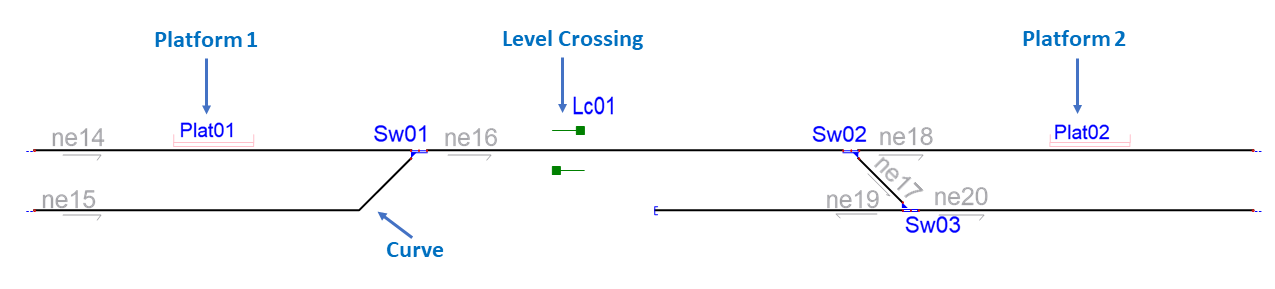
\includegraphics[width=1\textwidth]{resultados-obtenidos/ejemplo2/images/2_empty.png}
		\centering\caption{Topología ferroviaria del ejemplo 2 sin señalamiento.}
		\label{fig:EJ2_1}
	\end{figure}
	
	Para incrementar la dificultad del análisis y obtener resultados mas completos, se incluyeron curvas, finales de vías relativos y absolutos, junto con plataformas (Plat01, Plat02) y un cruce de vías (Lc01). La infraestructura se distribuyó de forma tal de tener que todos los elementos ferroviarios se encuentren aislados entre sí, separados por los cambios de vías.